\hsection{Floating Point Numbers}%
\label{sec:float}%
%
In the previous section, we have discussed integers in \python.
One of the very nice features of the \python~3 language is that integers can basically become arbitrarily large.
There is only the single type \pythonilIdx{int} and it can store any integer value, as long as the memory of our computer is large enough.%
%
\begin{sloppypar}%
In an ideal world, we would have a similar feature also for real numbers.
However, such a thing cannot be practically implemented.
You will certainly remember the numbers $\pi\approx3.141\decSep592\decSep653\decSep590\dots$ and $e\approx2.718\decSep281\decSep828\decSep459\dots$ from highschool maths.
They are transcendental~\cite{N1939TTOP,APM1991TOEAP,F2011TTOEAP}, i.e., their fractional digits never end and nobody has yet detected an orderly pattern in them.
Since these numbers are \inQuotes{infinitely long,} we would require infinitely much memory to store them \emph{if} we wanted to represent them \emph{exactly}.
So we don't and neither does \python.
We cannot really represent the real numbers~\realNumbers\ exactly in the memory of our computers.%
\end{sloppypar}%
%
\hsection{How Floating Point Numbers Work}%
\label{sec:howFloatingPointNumbersWork}%
%
\begin{figure}%
\centering%
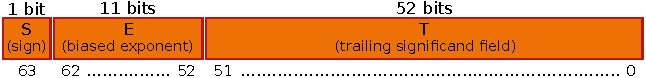
\includegraphics[width=0.7\linewidth]{\currentDir/floatIEEEStructure}%
\caption{The structure of an 64~bit / double precision IEEE~Standard 754 floating point number~\cite{IEEE2019ISFFPA,H1997IS7FPN}.}%
\label{fig:floatIEEEStructure}%
\end{figure}%
%
But how does it work in \python?
How can we deal with the fact that we cannot dynamically represent fractional numbers exactly even in typical everyday cases?
With \pythonilIdx{float}, \python\ offers us one type for fractional numbers.
This datatype represents numbers usually in the same internal structure as \pythonil{double}s in the \pgls{C}~programming language~\cite{PSF2024NTIFC}, which, in turn, internally have a 64~bit IEEE~Standard 754 floating point number layout~\cite{IEEE2019ISFFPA,H1997IS7FPN}.
The idea behind this standard is to represent both very large numbers, like~$10^{300}$ and very small numbers, like~$10^{-300}$.
In order to achieve this, the 64~bits are divided into three pieces, as illustrated in \cref{fig:floatIEEEStructure}.
%
\noviceHint{%
You just need to understand that \pythonilIdx{float}s have limited precision. %
You can jump right to the next section.}%
%
The first part, the so-called \pgls{significand} or \pgls{mantissa}, consists of 52~bits, represents the digits of the number.
52~bits can represent $52\log_2 10\approx 15$~to 16~decimal digits, meaning that we can represent numbers to a precision of about 15~digits.
If we would just use 52~bits, then this would limit us to represent numbers maybe from~$0$ to~$2^{52}-1$ at a resolution of~$1$.
Of course, we could also choose some other resolution, say~$0.001$.
In this case, we could represent numbers from~$0$ to $0.001*(2^{52}-1)$ and the smallest non-zero number would be~$0.001$ instead of~$1$.
Whatever fixed resolution we would choose, it would be good in some cases and bad in others.

Therefore, the second part of the 64~bit floating point number representation comes into play:
The 11~bits of the \pgls{exponent} represent a power of~2 which is multiplied to the \pgls{significand} to get the actual number.
In order to allow us to have both small and large numbers, this value must be able represent positive and negative exponents.
Therefore, the stored value of the \pgls{exponent} is taken and a \pgls{bias} of~1023 is subtracted.
Thus, a stored value of 2000 in the exponent fields leads to an actual exponent of $1050-1023=27$, which would mean that the \pgls{significand} is multiplied with~$2^{27}$, i.e., $134\decSep217\decSep728$.%
%
\begin{sloppypar}%
Finally, the \pgls{signBit} in the floating point number dataformat indicates whether the number is positive or negative.
Together, this allows us to represent numbers from $2.225\decSep073\decSep858\decSep507\decSep201\decSep4*10^{-308}$ to $1.797\decSep693\decSep134\decSep8623\decSep157*10^{308}$\pythonIdx{1.7976931348623157e+308}\pythonIdx{float!largest} with a resolution of approximately 15~digits.
Of course, the same range also applies to negative numbers and $0$~can be represented as well.
Indeed, there are even special floating point values for infinity and errors.
But more about this later.%
\end{sloppypar}%
%
Luckily, you will never really need to know these exact information.
The important thing to remember is:
Floating point numbers can represent a wide range of different values.
Their range is large but still limited.
They can represent integers and fractions.
However, their accuracy is always limited to about 15~digits.
In other words, regardless whether your \pythonilIdx{float} stores a very large or a very small number, you can have at most 15~digits of precision.
For example, adding~1 to~$10^{16}$ would still yield~$10^{16}$, because only 15~digits are \inQuotes{stored} and the~1 will just \inQuotes{fall off.}
You cannot represent numbers arbitrarily precisely.%
\endhsection%
%
\hsection{Floating Point Arithmetic}%
%
\begin{figure}%
\centering%
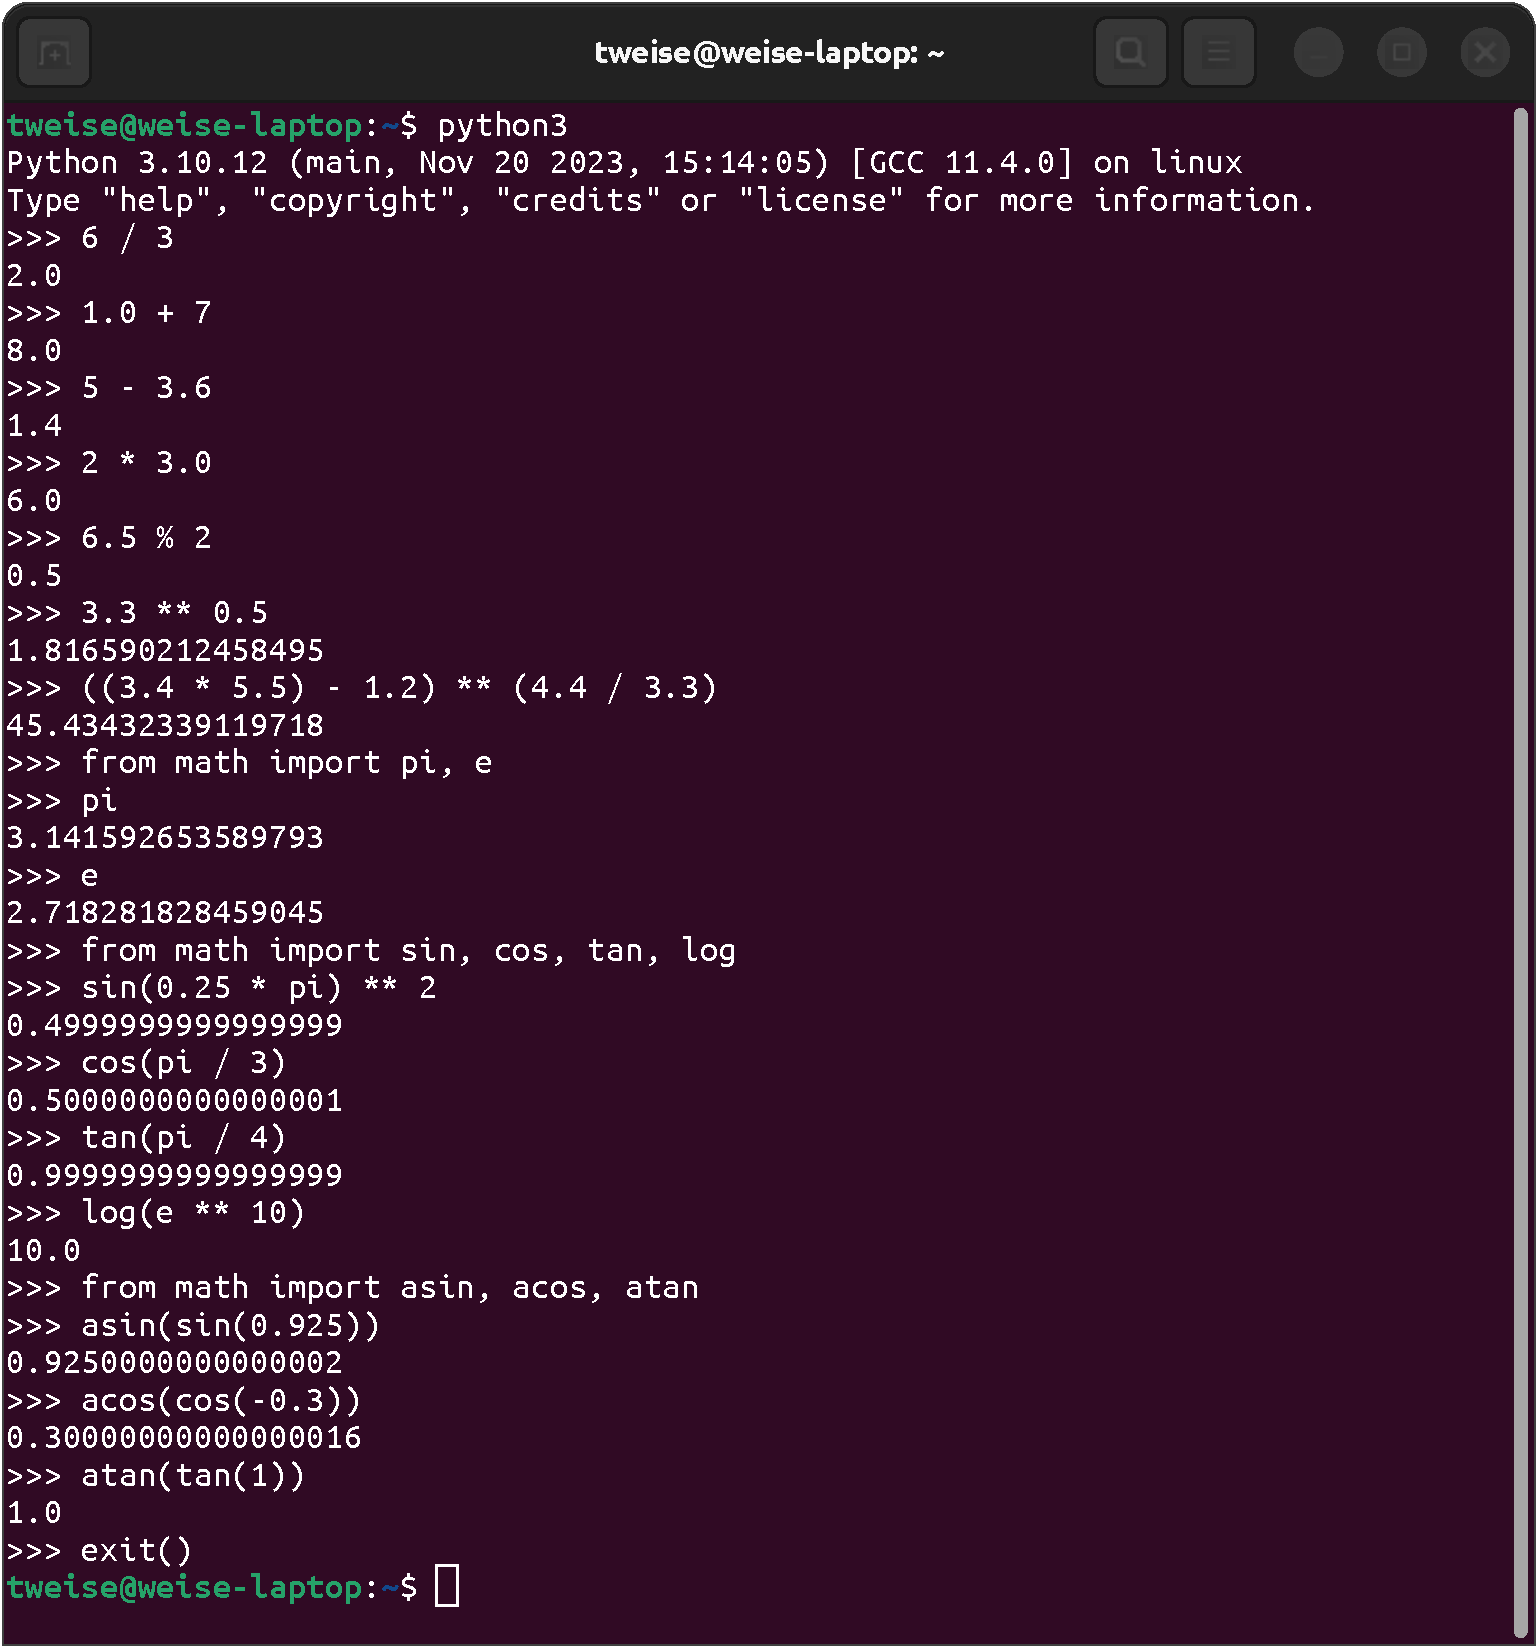
\includegraphics[width=0.8\linewidth]{\currentDir/floatMathInConsoleArith}%
\caption{Basic arithmetics with floating point numbers in \python.}%
\label{fig:floatMathInConsoleArith}%
\end{figure}%
%
Floating point numbers in \python\ can be distinguished from \pythonilIdx{int}s by having a decimal dot in their text representation, i.e., \pythonil{5.0} is a \pythonilIdx{float} and \pythonil{5} is an \pythonilIdx{int}.
Let us now look at some examples for the basic arithmetic operations available for \pythonilIdx{float}s in \cref{fig:floatMathInConsoleArith}.

We already learned that the division operator~\pythonilIdx{/} always yields a \pythonilIdx{float} result.
Therefore \pythonil{6 / 3} yields \pythonil{2.0} instead of \pythonil{2}.

The normal arithmetic operations like addition, subtraction, multiplication, division, and powers all work with \pythonilIdx{float}s as expected.
Remember, however, that if \pythonilIdx{float} and \pythonilIdx{int} numbers are mixed, the results are always \pythonilIdx{float}s.
Thus, \pythonil{1.0 + 7}\pythonIdx{+} gives us \pythonil{8} and \pythonil{2 * 3.0}\pythonIdx{*} yields \pythonil{6.0}.
In other words, if one \pythonilIdx{float} occurs somewhere in an expression, it will \inQuotes{infect} everything that it touches to become a \pythonilIdx{float} too, even if the result could be represented as \pythonilIdx{int}.
Some results cannot be integers anyway, for example \pythonil{5 - 3.6}\pythonIdx{-} evaluates to~\pythonil{1.4}.
The remainder (the modulo) of a division can also be computed for floating point numbers.
The remainder of the division of 6.5 by 2, i.e., \expandafter\pythonil{6.5 \% 2}\pythonIdx{\%} is~\pythonil{0.5}.%
%
\begin{sloppypar}%
The square root of 3.3 can be computed as $3.3^{0.5}$.
We can write this as \pythonil{3.3 ** 0.5}\pythonIdx{**}, which yields \pythonil{1.816590212458495}.
This brings us back to the previous section:
$\sqrt{3.3}$~is not actually 1.816\decSep590\decSep212\decSep458\decSep495.
It is an irrational number~\cite{S1988WPCHD,B1991IWNT} and irrational numbers cannot be expressed as fractions of integer numbers (by definition, otherwise they would be rational numbers).
Since they cannot be expressed as integer numbers, we cannot write them in any way like $\frac{1\decSep816\decSep590\decSep212\decSep458\decSep495\dots}{1\decSep000\decSep000\decSep000\decSep000\decSep000\dots}$, regardless of how large a denominator we would pick.
Hence, we cannot represent them exactly using discrete binary values of our computer's memory.
Hence, the floating point representation cuts off somewhere.
And this somewhere is after 15~decimal places.%
\end{sloppypar}%
%
\begin{sloppypar}%
We can of course also write and compute more complex mathematical expressions.
\pythonil{((3.4 * 5.5) - 1.2) ** (4.4 / 3.3)}\pythonIdx{(}\pythonIdx{)} corresponds to $((3.4*5.5)-1.2)^{\frac{4.4}{3.3}}$ and yields \pythonil{45.43432339119718}.
This is again not an exact value but a rounded value.
We always need to keep this in mind.%
\end{sloppypar}%
%
Let us recall our initial example of the transcendental irrational numbers~$\pi$ and~$e$.
Certainly, these are very important constants that would be used in many computations.
We can make them accessible in our code by importing them from the \pythonilIdx{math} module.\footnote{%
We will learn about these mechanism in detail later on.}
This can be done by typing \pythonil{from math import pi, e}\pythonIdx{import}\pythonIdx{from}\pythonIdx{math}.
When we then type \pythonilIdx{pi} and \pythonilIdx{e}, we can get to see their value in floating point representations: \pythonil{3.141592653589793} and \pythonil{2.718281828459045}, respectively.
Again, these are not the exact values, but they are as close as we can get in this format.

Of course, $\pi$ and~$e$ alone are not that much useful.
If you reach back into your highschool days again, you will remember many interesting functions that are related to them.
Let us import a few of them, again from the \pythonilIdx{math} module, via \pythonil{from math import sin, cos, tan, log}\pythonIdx{sin}\pythonIdx{cos}\pythonIdx{tan}\pythonIdx{log}.
I think you can guess what these functions do.

From highschool, you may remember that~$\sin{\frac{\pi}{4}}=\frac{\sqrt{2}}{2}$ and thus~$\sin^2{\frac{\pi}{4}}=0.5$.
Let us compute this in \python\ by doing \pythonil{sin(0.25 * pi) ** 2}\pythonIdx{sin}.
Surprisingly, we get \pythonil{0.4999999999999999} instead of \pythonil{0.5}.
The reason is again the limited precision of \pythonilIdx{float}, which cannot represent~$\frac{\sqrt{2}}{2}$ exactly.
Similarly, $\cos{\frac{\pi}{3}}=\frac{1}{2}$ but \pythonil{cos(pi / 3)}\pythonIdx{cos} yields \pythonil{0.5000000000000001} and $\tan{\frac{\pi}{4}}$ expressed as \pythonil{tan(pi / 4)}\pythonIdx{tan} returns \pythonil{0.9999999999999999} instead of~$1$.
Then again, these values are incredibly close to the exact results.
They are off by \emph{less than~$10^{-15}$} so for all practical concerns, they are close enough.
Sometimes, we even get the accurate result, e.g., when computing $\ln(e^{10})$ by evaluating \pythonil{log(e ** 10)}\pythonIdx{log}, which results in~\pythonil{10.0}.

As final example for floating point arithmetics, let us import the inverse trigonometric functions by doing \pythonil{from math import asin, acos, atan}\pythonIdx{math}\pythonIdx{asin}\pythonIdx{acos}\pythonIdx{atan}.
Obviously, $\arcsin{\sin{0.925}}$ should be~$0.925$.
Calculating \pythonil{asin(sin(0.925))}\pythonIdx{asin}\pythonIdx{sin} indeed yields~\pythonil{0.9250000000000002}.
Due to the periodicity of the trigonometric functions, $\arccos{\cos{-0.3}}$ is~$0.3$ and \pythonil{acos(cos(-0.3))}\pythonIdx{acos}\pythonIdx{cos} results in~\pythonil{0.30000000000000016}.
For $\arctan{\tan{1}}$ we even get the exact result \pythonil{1.0} by computing \pythonil{atan(tan(1))}\pythonIdx{atan}\pythonIdx{tan}.%
\endhsection%
%
\hsection{Back to Integers: Rounding}%
%
\begin{figure}%
\centering%
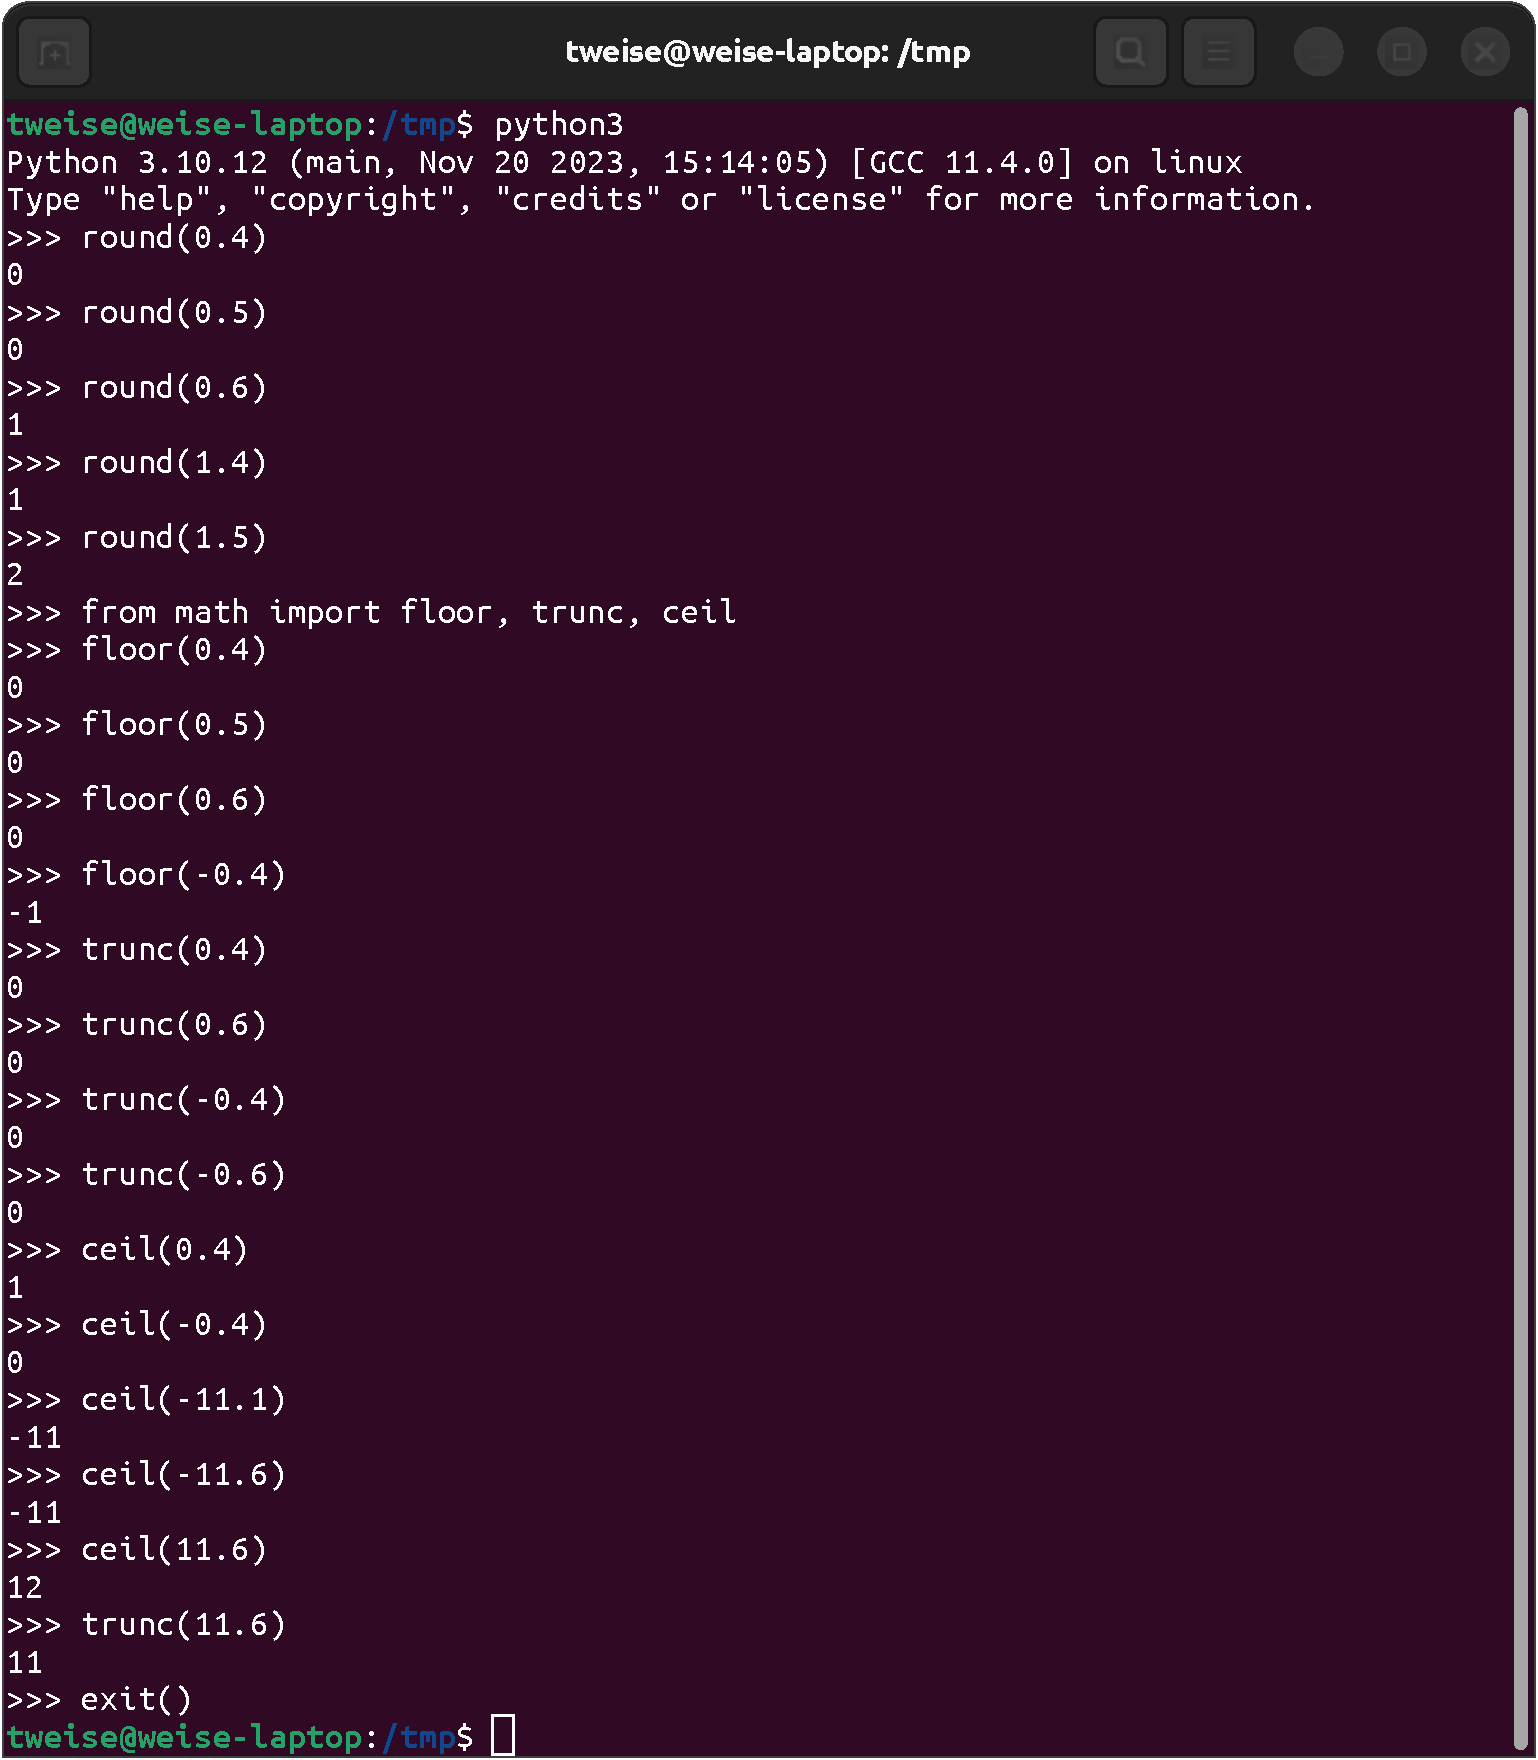
\includegraphics[width=0.8\linewidth]{\currentDir/floatMathInConsoleRound}%
\caption{Rounding \pythonilIdx{float} values to \pythonilIdx{int} values.}%
\label{fig:floatMathInConsoleRound}%
\end{figure}%
%
We already learned that a single \pythonilIdx{float} value inside a computation that otherwise uses \pythonilIdx{int}s basically forces the whole result to become a \pythonilIdx{float} as well.
But maybe sometimes we want to have an \pythonilIdx{int} as result.
Therefore, we need a \inQuotes{way back} from \pythonilIdx{float} to \pythonilIdx{int}.
\python\ offers several functions for this.

The first and maybe most common one is \pythonilIdx{round}.
This function accepts a \pythonilIdx{float} and rounds it to the nearest integer.
If two integer numbers are equally close, it rounds it to the one that is even.
This can be very surprising, as we learned in school that $x.5$ should be rounded to $x+1$.
This will only happen with \pythonilIdx{round} if $x+1$~is even.
We find examples for the behavior of \pythonilIdx{round} in \cref{fig:floatMathInConsoleRound}.
\pythonil{round(0.4)} yields the integer~\pythonil{0}, as expected.
\pythonil{round(0.5)} returns~\pythonil{0} as well, which one may not expect -- but \pythonil{0} is even and \pythonil{1} would be odd.
\pythonil{round(0.6)} gives us the integer~\pythonil{1}.
If we compute \pythonil{round(1.4)}, we still get~\pythonil{1}.
However, doing \pythonil{round(1.5)} gives us~\pythonil{2}.
This is because \pythonil{2} is even.

Three more common functions to turn \pythonilIdx{float}s to \pythonilIdx{int}s are given in the \pythonilIdx{math} module.
We can import them via \pythonil{from math import floor, trunc, ceil}\pythonIdx{from}\pythonIdx{import}\pythonIdx{math}\pythonIdx{floor}\pythonIdx{trunc}\pythonIdx{ceil}.
(Again, we will learn later how \pythonilIdx{import} actually works.
For now, just accept that it makes some functions available.)

\pythonilIdx{floor} rounds the \pythonilIdx{float} it receives to the nearest integer which is less than or equal to.
\pythonil{floor(0.4)}, \pythonil{floor(0.5)}, and \pythonil{floor(0.6)} all yield \pythonil{0}.
\pythonil{floor(-0.4)} gives us \pythonil{-1}.

\pythonilIdx{trunc} just discards any fractional digits and only returns the integer part of a number.
Hence, \pythonil{trunc(-0.6)}, \pythonil{trunc(-0.4)}, \pythonil{trunc(0.4)}, and \pythonil{trunc(0.6)} all yield~\pythonil{0}.

Finally, \pythonilIdx{ceil} rounds to the nearest integer which is greater than or equal to its argument.
\pythonil{ceil(0.4)} yields \pythonil{1} and \pythonil{-0.4} results in~\pythonil{0}.
\pythonil{ceil(-11.1)} and \pythonil{ceil(-11.6)} both result in \pythonil{11}.
\pythonil{ceil(11.6)} gives us~\pythonil{12}.

You can also try to directly convert any datatype (that supports it) to an \pythonilIdx{int}.
This works by simply putting it as argument to the function \pythonilIdx{int}.
With \pythonilIdx{float}s, this works exactly as invoking \pythonilIdx{trunc}:
\pythonil{int(0.9)} and \pythonil{int(-0.9)} both give us~\pythonil{1}.
\pythonil{11.6} yields~\pythonil{11}.

With this, we have several ways to turn \pythonilIdx{float}s to \pythonilIdx{int}s.
However, especially with the function \pythonilIdx{round}, we need to be careful.
It does \emph{not} work as one would expect!%
%
\endhsection%
%
\hsection{The Scientific Notation}%
\label{sec:scientificNotation}%
%
\begin{figure}%
\centering%
\begin{tabular}{r@{}r@{{\color{orange}\textbf{e}}}l@{~~$\equiv$~~}r@{}l}%
\multicolumn{2}{c}{$\beta$}&$\gamma$&\multicolumn{2}{c}{$\alpha$}\\\hline%
&\texttt{A.BCDEFG}{\dots}&\texttt{\color{red}{+}}\texttt{HIJ}&&$\texttt{A.BCDEFG}{\dots}*{\color{orange}10}^{HIJ}$\\
&\texttt{A.BCDEFG}{\dots}&\texttt{\color{red}{-}}\texttt{HIJ}&&$\texttt{A.BCDEFG}{\dots}*{\color{orange}10}^{{\color{red}{-}}HIJ}$\\
{\color{blue}{-}}&\texttt{A.BCDEFG}{\dots}&\texttt{\color{red}{+}}\texttt{HIJ}&${\color{blue}{-}}$&$\texttt{A.BCDEFG}{\dots}*{\color{orange}10}^{HIJ}$\\
{\color{blue}{-}}&\texttt{A.BCDEFG}{\dots}&\texttt{\color{red}{-}}\texttt{HIJ}&${\color{blue}{-}}$&$\texttt{A.BCDEFG}{\dots}*{\color{orange}10}^{{\color{red}{-}}HIJ}$%
\end{tabular}%
%
\caption{The structure of the scientific notation for floating point numbers in \python, which represent a value~$\alpha$ in the form~$\beta*10^{\gamma}$.}%
\label{fig:scientificNotation}%
\end{figure}%
%
\begin{figure}%
\centering%
%
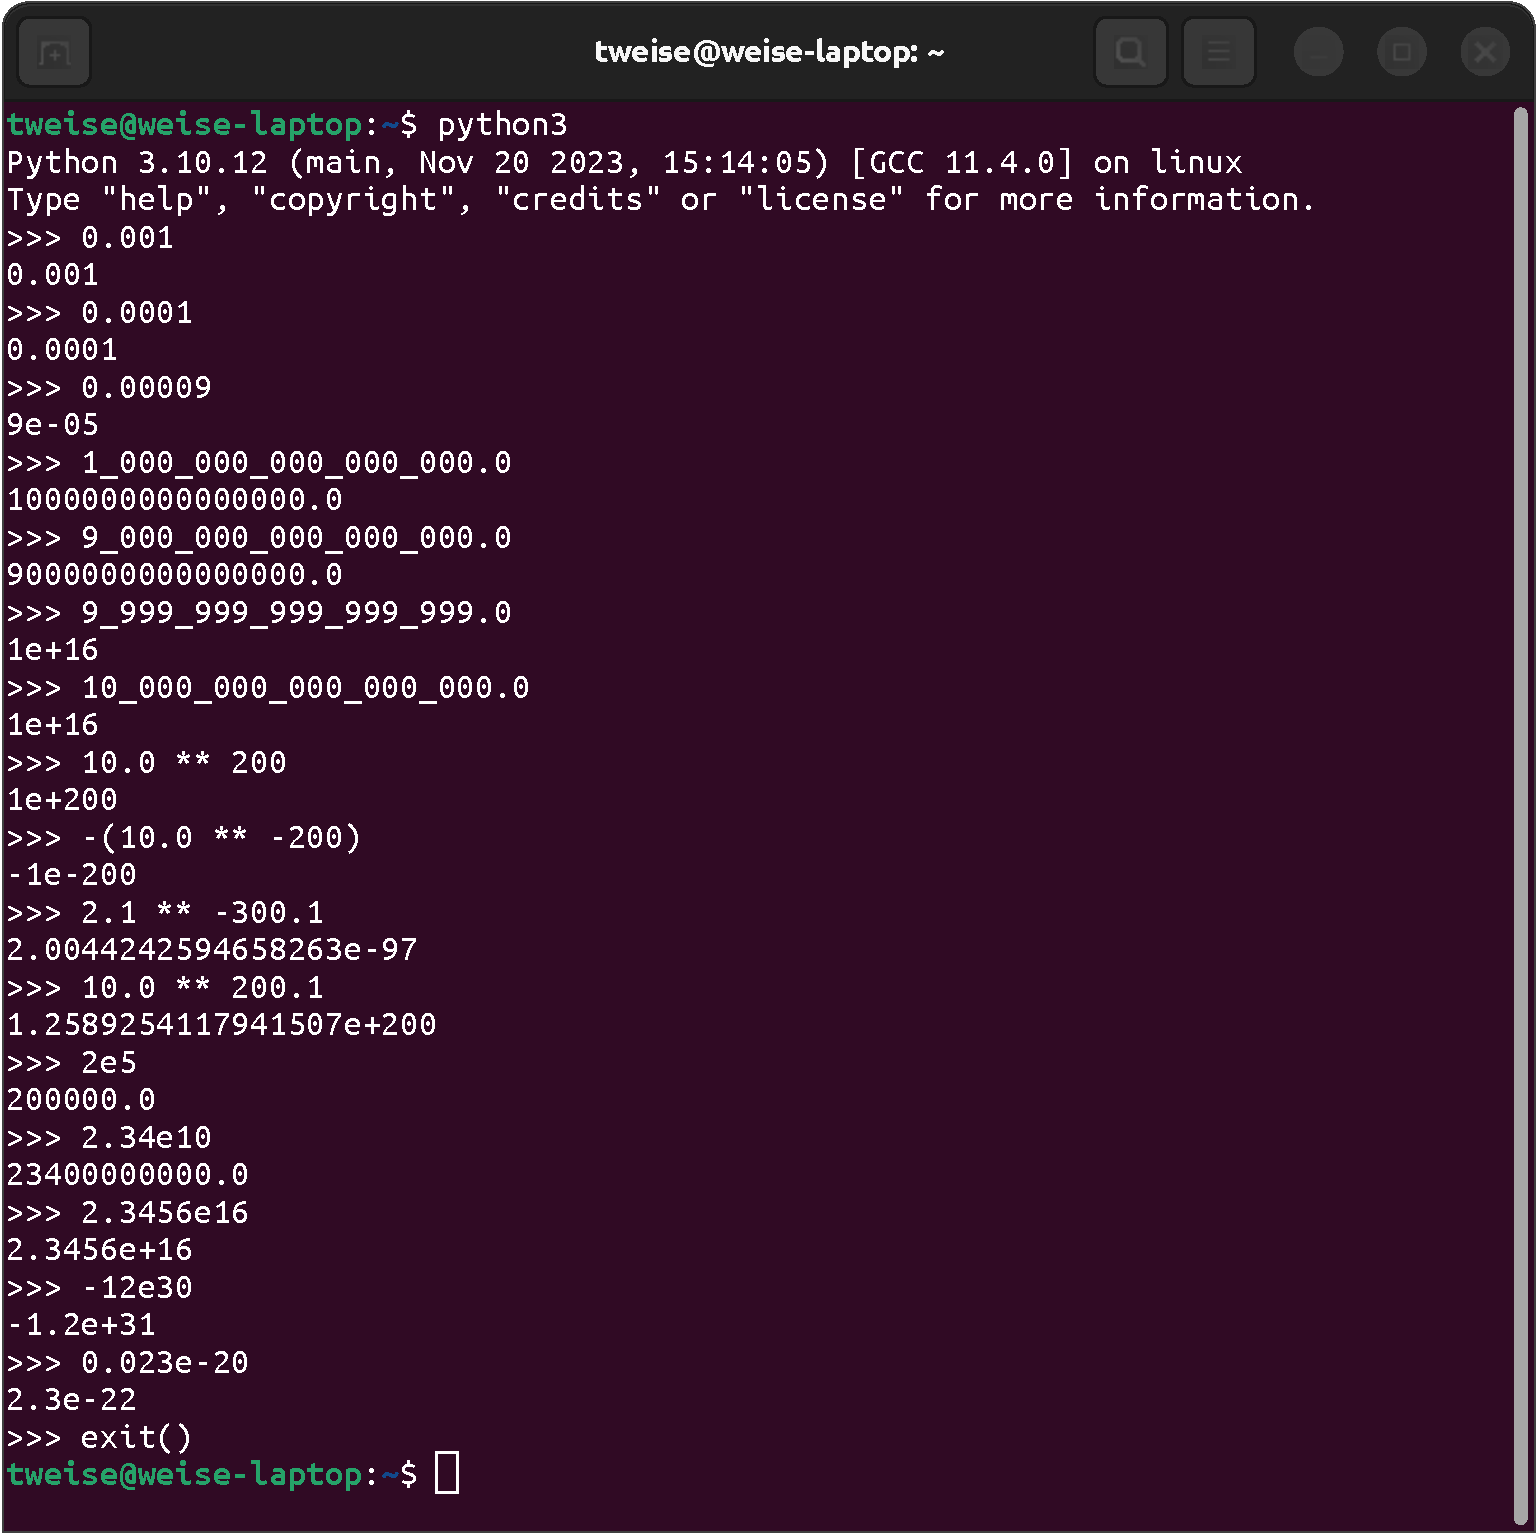
\includegraphics[width=0.8\linewidth]{\currentDir/floatMathInConsoleSciNot}%
\caption{Examples for the scientific notation in \python.}%
\label{fig:floatMathInConsoleSciNot}%
\end{figure}%
%
Earlier on, we wrote that \pythonilIdx{float}s can represent numbers as large as~$10^{300}$ or as small as~$10^{-300}$.
This leads to the question how it would print such values on the console and how we can read them.
While it would be hugely impractical to write a~1 followed by 300~zeros to represent~$10^{300}$, it would also be \emph{wrong}.
We also already know the reason for this:
A \pythonilIdx{float} is accurate to 15~decimals.
So basically, the first 15~zeros would be correct, but the values of the other digits are actually \emph{undefined}.

\python, like many programming languages, solves this problem by using the \emph{scientific notation} for floating point numbers.
It uses this notation for any (absolute) \pythonilIdx{float} value smaller than~$10^{-4}$ or larger than or equal to~$10^{16}$.
Such numbers~$\alpha$ are then represented in the form~$\beta*10^{\gamma}$ (such that $\beta*10^{\gamma}=\alpha$, obviously).
Since we cannot write this so nicely in a console, a lowercase~\texttt{e} takes the place of the~$10$ and $\beta$ and $\gamma$ are written as normal text.
In order to make sure that each number~$\alpha$ has unique representation, it is defined that $\alpha$ must have exactly one non-zero leading digit, which may be followed by a decimal dot and then a fractional part.
This notation is illustrated in \cref{fig:scientificNotation}.
\emph{This notation only applies to \pythonilIdx{float}s, \textbf{not} \pythonilIdx{int}s.}

In \cref{fig:floatMathInConsoleSciNot} we provide some examples for this notation.
When we write \pythonil{0.001} or \pythonil{0.0001} in a \python\ console, the output is still this same number.
However, \pythonil{0.00009} is presented as \pythonil{9e-05}, which stands for~$9*10^{-5}$.%
%
\begin{sloppypar}%
Did you know that you are allowed to insert underscores (\pythonil{_}\pythonIdx{\_}) anywhere in a number as a visual aid?
If not, you know now.
We can write $10^{15}$ as \pythonilIdx{float} by typing \pythonil{1_000_000_000_000_000.0}.
This equals the much less readable \pythonil{1000000000000000.0}.
We can do the same for $9*10^{15}$ by writing \pythonil{9_000_000_000_000_000.0} and get \pythonil{9000000000000000.0}.
However, if we write \pythonil{9_999_999_999_999_999.0}, something interesting happens:
We get \pythonil{1e+16}, i.e., $10^{16}$.
This is because of the limited precision of the floating point numbers, namely the 15~digits often mentioned above.
We cannot distinguish $10^{16}$ and $10^{16}-1$ when using \python's \pythonilIdx{float}s.
Indeed, writing \pythonil{10_000_000_000_000_000.0} also yields \pythonil{1e+16}.%
\end{sloppypar}%
%
This notation can also show really big numbers.
For example $10^{200}$, i.e., \pythonil{10.0 ** 200}, shows up as \pythonil{1e+200}.
The really really small number $-10^{-200}$ in turn, computed via \pythonil{-(10.0 ** -200)}, is denoted as \pythonil{-1e-200}.

The numbers are always scaled such that they begin with non-zero digit followed by the fractional part separated with a decimal dot, if need be.
Examples for this are \pythonil{2.1 ** -300.1} which yields \pythonil{2.0044242594658263e-97} and \pythonil{10.0 ** 200.1}, which turns up as \pythonil{1.2589254117941507e+200}.

Of course, you can also input numbers in scientific notation.
If you write \pythonil{2e5}, this turns into \pythonil{200000.0}.
Of course, the number is stored as a \pythonilIdx{float} internally and this \pythonilIdx{float} does not know from which kind of text it was created.
When it is turned back into text, it becomes a \inQuotes{normal number,} because it is less than~$10^{16}$.
And so does \pythonil{2.34e10}, which becomes \pythonil{23400000000.0}.
\pythonil{2.3456e16} however indeed remains \pythonil{2.3456e16}.

You can even violate the scientific notation a bit when entering numbers if you feel naughty.
\pythonil{-12e30}, for example, would better be written as \pythonil{-1.2e+31}, which the \python\ console will do for you in its output.
Similarly, \pythonil{0.023e-20} becomes \pythonil{2.3e-22}.
\endhsection%
%
\hsection{Limits and Special Floating Point Values: Infinity and \inQuotes{Not a Number}}%
\label{sec:float:special}%
%
\begin{figure}%
\centering%
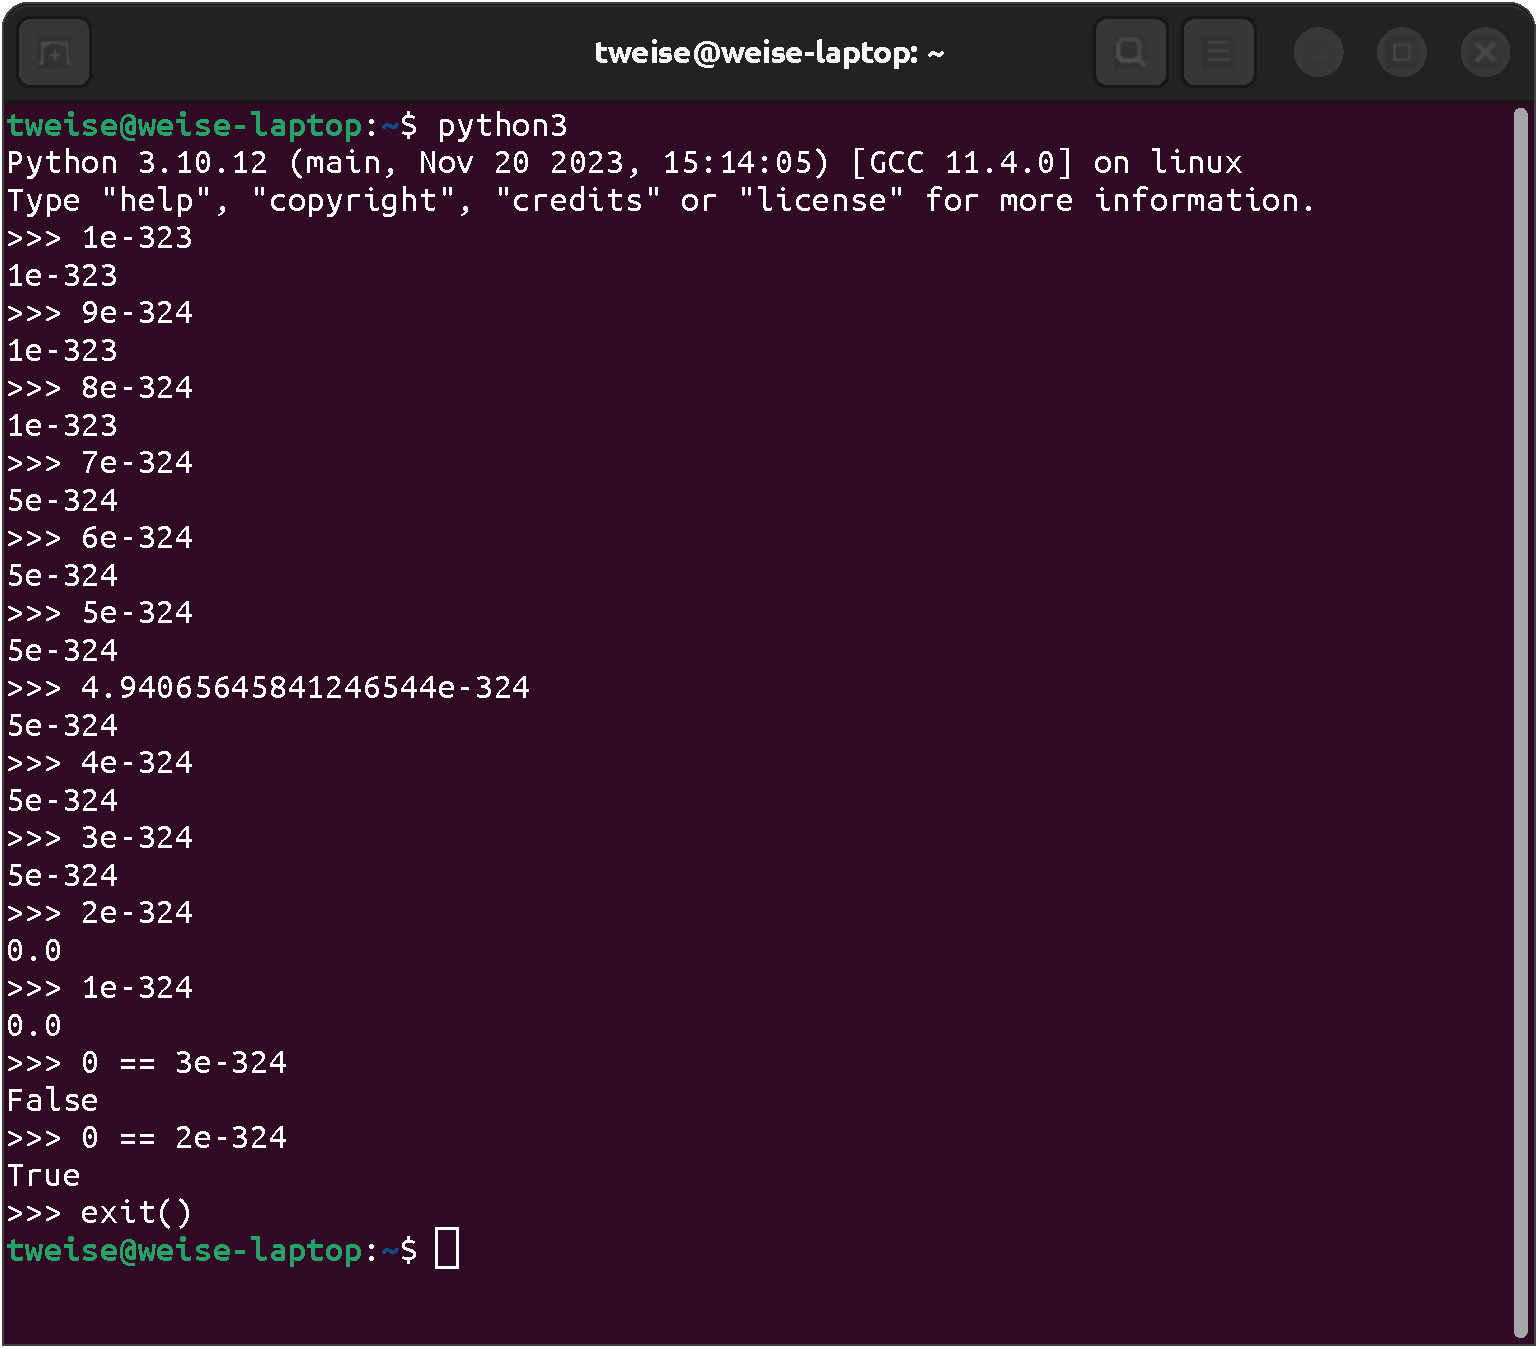
\includegraphics[width=0.7\linewidth]{\currentDir/floatMathInConsoleZero}%
\caption{What happens with very small floating point numbers in \python?\pythonIdx{0.0}}%
\label{fig:floatMathInConsoleZero}%
\end{figure}%
%
We already learned that the floating point type \pythonilIdx{float} can represent both very small and very large numbers.
But we also know that it is internally stored as chunk of 64~bits.
So its range must be somehow finite.
What happens if we exceed this finite range?

First the easy part:
Now, we said that \python\ can store very small numbers, like $10^{-300}$, in the \pythonilIdx{float} datatype.
But how small really?
Finding this out from the documentation is actually not so easy.
Luckily, \pgls{Java} uses the same standard for its class \pythonil{Double}.
In its documentation~\cite{O2024CD}, we find that the minimum value is~$2^{-1074}$, which is approximately~$4.940\decSep656\decSep458\decSep412\decSep465\decSep44*10^{-324}$.
So we would expect the smallest possible floating point value in \python\ to also be in this range.

In \cref{fig:floatMathInConsoleInf}, we take a look what happens if we approach this number.
We use the scientific notation and begin to print the number~\pythonil{1e-323} (which is~$10^{-323}$).
This number is correctly represented as \pythonilIdx{float} and shows up in the console exactly as we wrote it.
However, if we go a bit smaller and enter \pythonil{9e-324}, which is~$9*10^{-324}=0.9*10^{-323}$, we find that it again shows up in the console as \pythonil{1e-323}.
This is because the number is already subnormal~\cite{IEEE2019ISFFPA,H1997IS7FPN}, i.e., uses only a few of the significand bits.
The full precision of 15~digits is no longer available at this small scale.
Thus \pythonil{9e-324} and \pythonil{1e-323} map to the same \pythonilIdx{float}.
Converting this \pythonilIdx{float} to text yields \pythonil{'1e-323'}.
The same happens for \pythonil{8e-324}, which also maps to \pythonil{1e-323}.
\pythonil{7e-324}, however, is the same as \pythonilIdx{5e-324}\pythonIdx{float!smallest}.
Matter of fact, \pythonil{6e-324}, \pythonilIdx{5e-324}, \pythonil{4e-324}, and \pythonil{3e-324} all map to this same \pythonilIdx{float}\pythonIdx{float!smallest}.

It turns out that this number is already the smallest \pythonilIdx{float} that can be represented:
\pythonil{2e-324} simply becomes \pythonilIdx{0.0}.
This value is simply too small to be represented as a 64~bit / double precision IEEE~Standard 754 floating point number~\cite{IEEE2019ISFFPA,H1997IS7FPN}.
The text \pythonil{2e-324} that we enter into the \python\ console will therefore be translated to the \pythonilIdx{float}~\pythonil{0.0}.
The comparison \pythonil{2e-324 == 0.0}\pythonIdx{==} therefore results in \pythonilIdx{True}, while \pythonil{3e-324 == 0.0} is still \pythonilIdx{False}.\footnote{%
See \cref{sec:bool} for more information on comparisons and the \pythonilIdx{bool} datatype with its values \pythonilIdx{True} and \pythonilIdx{False}.%
}
So we learned what happens if we try to define very small floating point numbers:
They become zero.

\begin{figure}%
\centering%
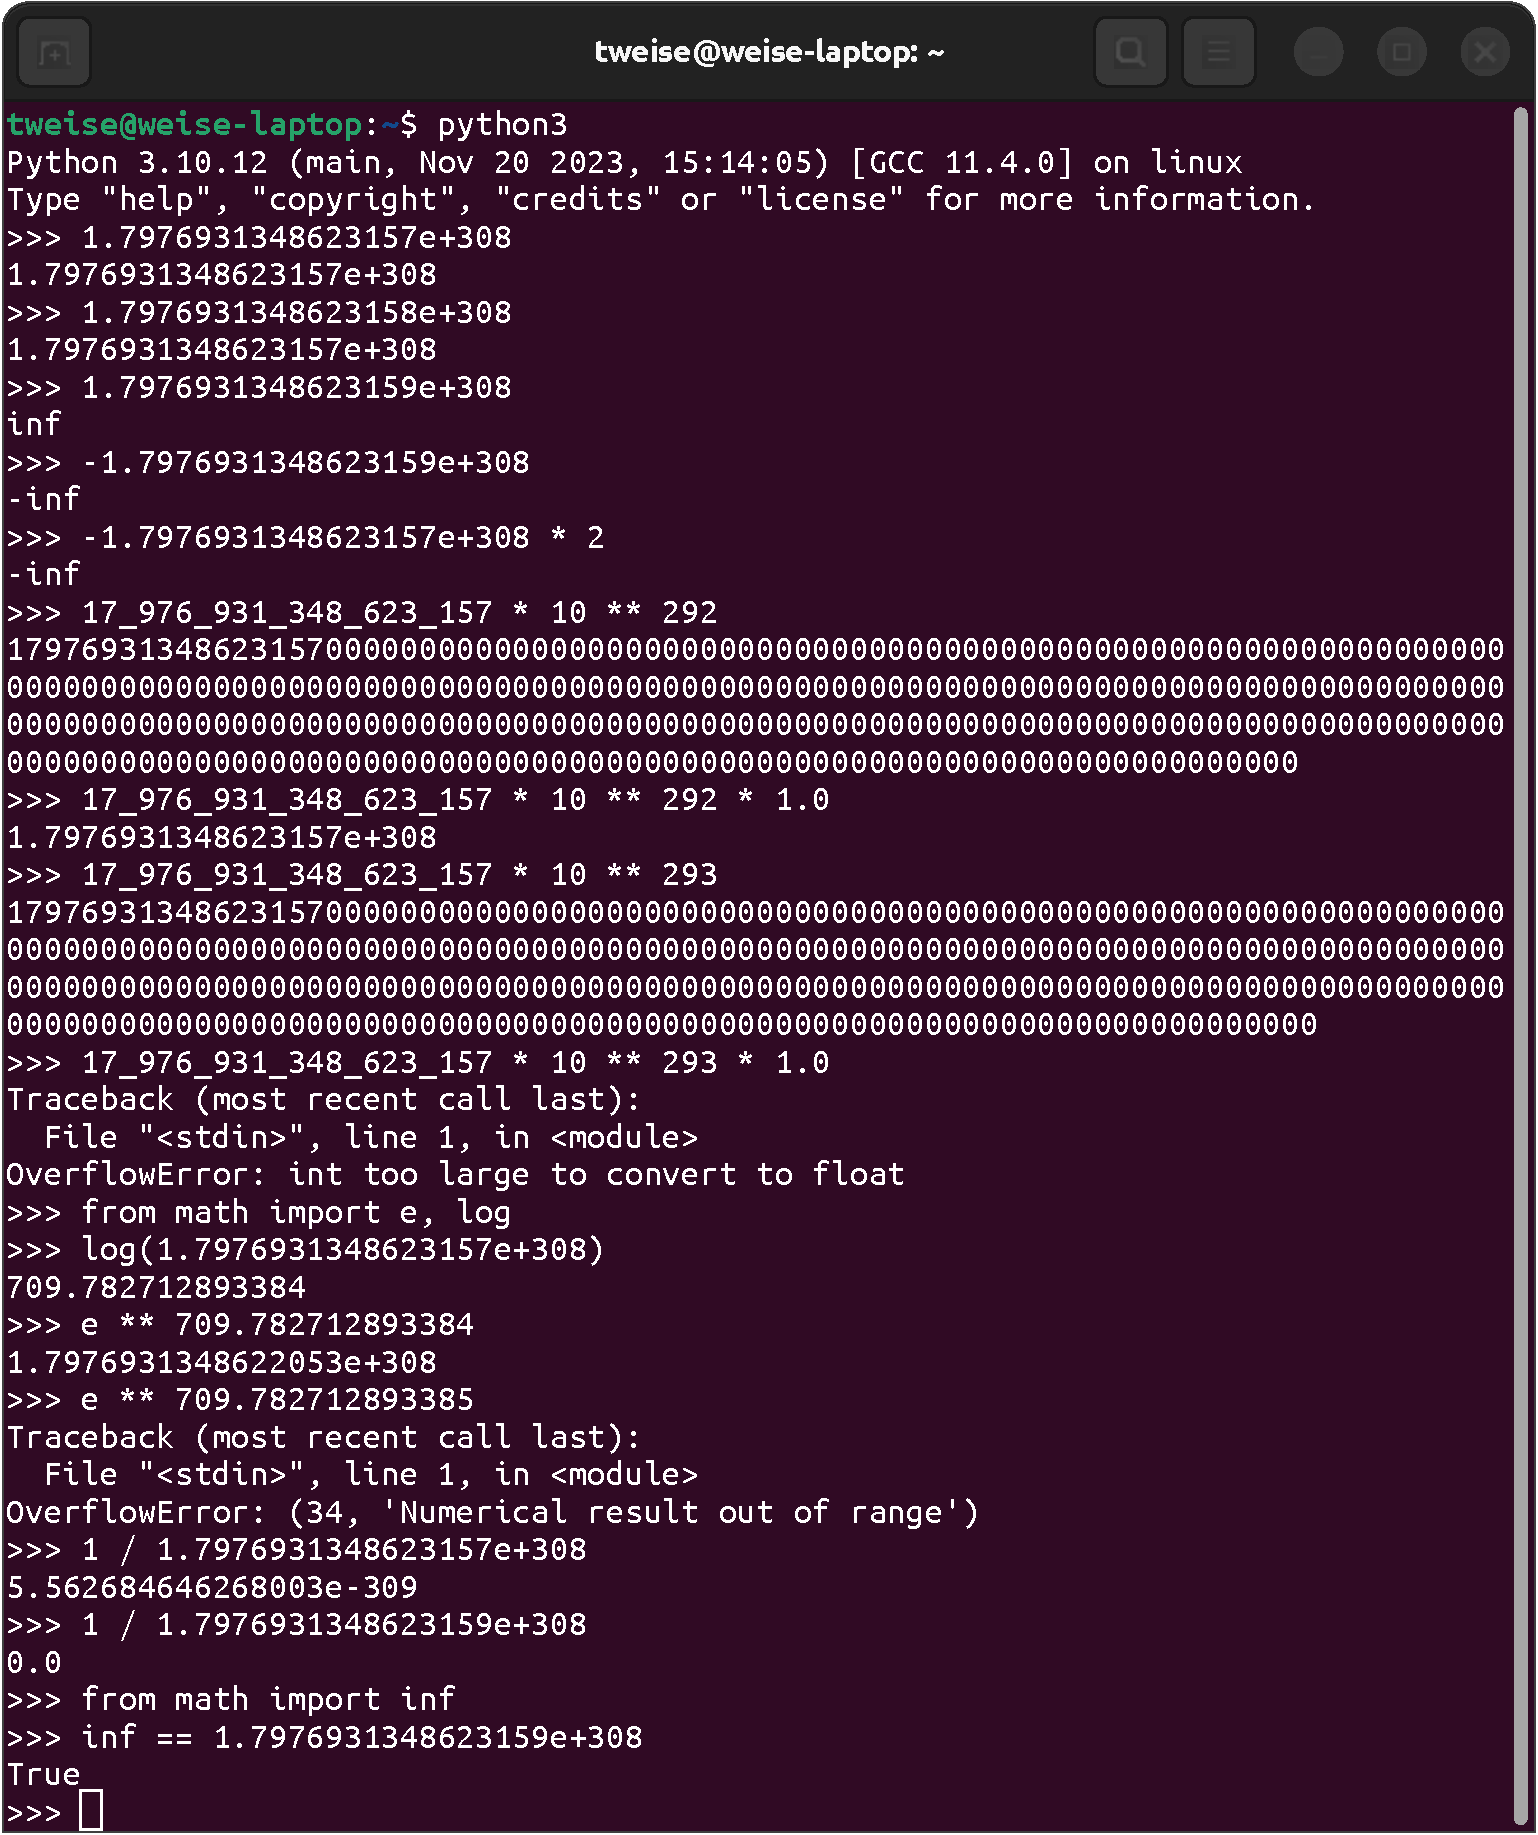
\includegraphics[width=0.7\linewidth]{\currentDir/floatMathInConsoleInf}%
\caption{What happens with very large floating point numbers in \python?\pythonIdx{inf}}%
\label{fig:floatMathInConsoleInf}%
\end{figure}%

But what happens to numbers that are too big for the available range?
Again, according to the nice documentation of \pgls{Java}, the maximum 64~bit double precision floating point number value is~$(2-2^{-52})*2^{1023}\approx1.797\decSep693\decSep134\decSep862\decSep315\decSep708\dots*10^{308}$.
We can enter this value as \pythonilIdx{1.7976931348623157e+308}\pythonIdx{float!largest} and it indeed prints correctly in \cref{fig:floatMathInConsoleInf}.
If we step it up a little bit and enter \pythonil{1.7976931348623158e+308}, due to the limited precision, we again get \pythonilIdx{1.7976931348623157e+308}\pythonIdx{float!largest}.
However, if we try entering \pythonil{1.7976931348623159e+308} into the \python\ console, something strange happens:
The output is \pythonilIdx{inf}.
\pythonil{-1.7976931348623159e+308} gives us \pythonilIdx{-inf}.
Multiplying this value by two, i.e., computing \pythonil{-1.7976931348623157e+308 * 2}, still yields \pythonil{-inf}.
Intuitively, based on its name, one would assume that \pythonilIdx{inf} stands for \inQuotes{infinity} or~$\infty$.
However, it \emph{actually} means \emph{too big to represent as \pythonilIdx{float} or~$\infty$}.
If we enter numbers that are too big or exceed the valid range of \pythonilIdx{float} by multiplication, addition, subtraction, or division, we simply get~\pythonilIdx{inf}.
This does not actually mean \inQuotes{mathematical infinity,} because, while \pythonil{-1.7976931348623159e+308}\pythonIdx{float!largest} is very big, it is not infinitely big.
It simply means that the number is too big to put it into a 64~bit \pythonilIdx{float}.

Actually, the \pythonilIdx{int} type can represent larger numbers easily.
\pythonilIdx{1.7976931348623157e+308}\pythonIdx{float!largest} is equivalent to \pythonil{17_976_931_348_623_157 * 10 ** 292}.
This prints as a number with many zeros.
Multiplying it with \pythonil{1.0} yields a \pythonilIdx{float} with value \pythonilIdx{1.7976931348623157e+308}\pythonIdx{float!largest}, exactly as expected.
If we try a number ten times as large, i.e., \pythonil{17_976_931_348_623_157 * 10 ** 293}, this is no problem with the \pythonilIdx{int}.
But we can no longer convert it to a \pythonilIdx{float} by multiplying with~\pythonil{1.0}.
Trying to do that with a ten times larger number, i.e., computing \pythonil{17_976_931_348_623_157 * 10 ** 293 * 1.0} leads to an exception:
The output is \pythonil{OverflowError: int too large to convert to float}\pythonIdx{OverflowError}.
An exception terminates the current flow of execution and signals an error.
We will learn later what exceptions actually are and how to handle them properly.

The important thing to realize is that an overflow of a \pythonilIdx{float} may either lead to the \pythonilIdx{inf} value or to an error that stops your computation from continuing.
As another example, let us again import the natural logarithm function \pythonilIdx{log} and the Euler's constant~\pythonilIdx{e} from the \pythonilIdx{math} module by doing \pythonil{from math import e, log}\pythonIdx{from}\pythonIdx{math}\pythonIdx{import}.
We now can compute the natural logrithm from the largest possible \pythonilIdx{float} via \pythonil{log(1.7976931348623157e+308)}.
We get \pythonil{709.782712893384}.
Raising~$e$ to this power by doing \pythonil{e ** 709.782712893384} leads to the slightly smaller number~\pythonil{1.7976931348622053e+308} due to the limited precision of the \pythonilIdx{float} type.
However, if we try to raise~$e$ to a slightly larger power, and, for example, try to do \pythonil{e ** 709.782712893385}, we again face an \pythonilIdx{OverflowError}.

We can also try to divide~1 by the largest \pythonilIdx{float} and do \pythonil{1 / 1.7976931348623157e+308}\pythonIdx{/}.
The result is the very small number \pythonil{5.562684646268003e-309}.
However, if we divide~1 by \pythonil{1.7976931348623159e+308}, we get~\pythonil{0.0}.
The reason is that \pythonil{1.7976931348623159e+308} becomes \pythonilIdx{inf} and \pythonil{1 / inf}\pythonIdx{/} is~\pythonilIdx{0.0}.

Finally, \pythonilIdx{inf} also exists as constant in the \pythonilIdx{math} module.
We can import it via \pythonil{from math import inf}\pythonIdx{inf}.
And indeed, since the text \pythonil{1.7976931348623159e+308} is parsed to a \pythonilIdx{float} value of \pythonilIdx{inf}, we find that \pythonil{1.7976931348623159e+308 == inf} yields~\pythonilIdx{True}.

\begin{figure}%
\centering%
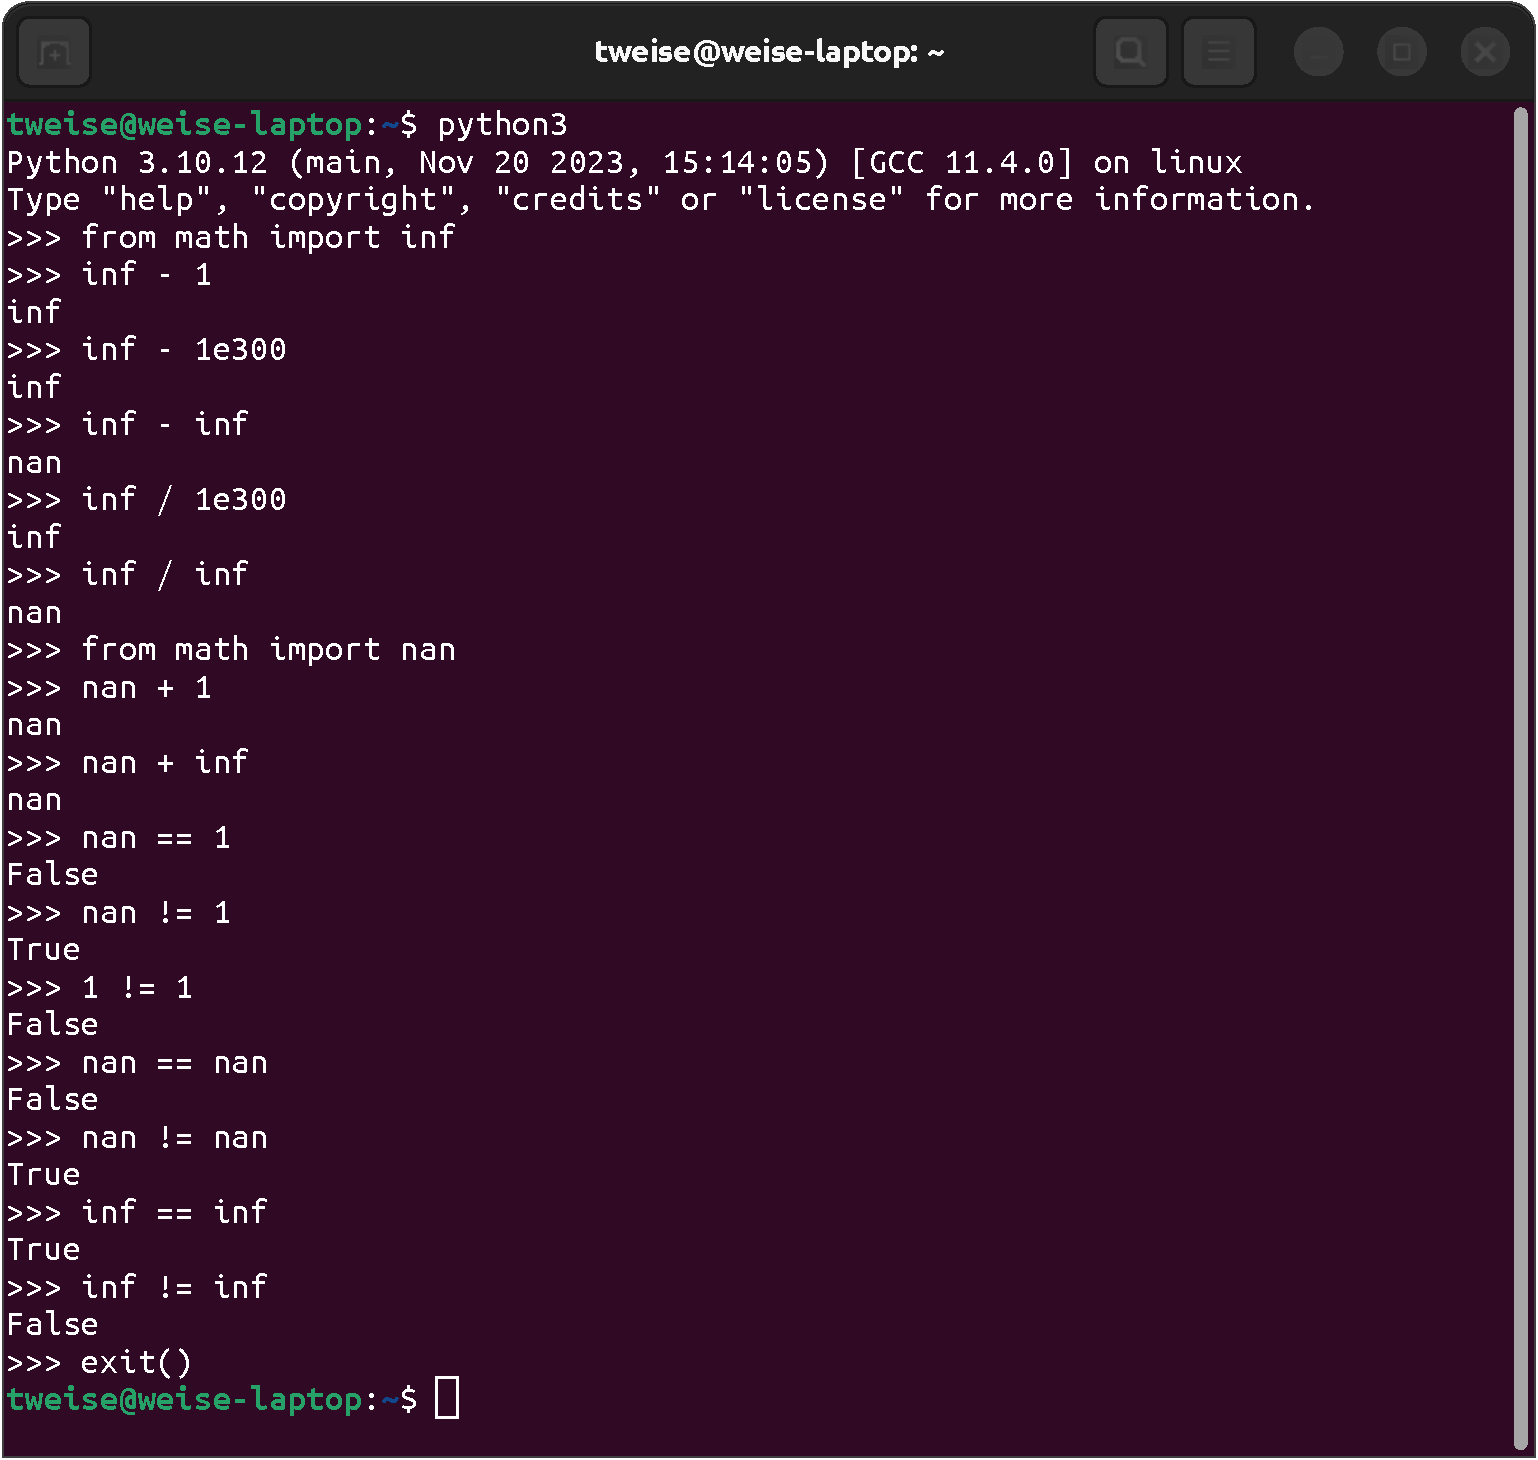
\includegraphics[width=0.8\linewidth]{\currentDir/floatMathInConsoleNaN}%
\caption{Not a Number\pythonIdx{Not a Number}, i.e., \pythonilIdx{nan}.}%
\label{fig:floatMathInConsoleNaN}%
\end{figure}%

Now, \pythonilIdx{inf} not actually being~$\infty$ is a little bit weird.
But it can get even stranger, as you will see in \cref{fig:floatMathInConsoleNaN}.
\pythonilIdx{inf} is a number which is too big to be represented as \pythonilIdx{float} \emph{or}~$\infty$.
So it is natural to assume that \pythonil{inf - 1} remains \pythonilIdx{inf} and that even \pythonil{inf - 1e300} remains \pythonilIdx{inf} as well.
However, what is \pythonil{inf - inf}?
Mathematically speaking, this is very dodgy and $\infty-\infty$ as such is not a thing.
Or \emph{not a number}\pythonIdx{Not a Number}.
Or \pythonilIdx{nan}, which stands for, well, Not a Number\pythonIdx{Not a Number}.

\pythonilIdx{nan} means that the result of a computation is neither a finite number or infinite.
It is the result of shenanigans such as \pythonil{inf - inf} or \pythonil{inf / inf}.
A \pythonilIdx{nan} value anywhere in a computation infects the result of the computation to also become \pythonilIdx{nan}.
\pythonil{nan + 1} remains \pythonilIdx{nan} and so does \pythonil{nan + inf}.

The value \pythonilIdx{nan} is different from \emph{any} value.
\pythonil{nan == 1} is \pythonilIdx{False} and \pythonil{nan != 1} is \pythonilIdx{True} (\pythonilIdx{!=} checks for inequality).
While all other float values are equal to themselves and -- therefore -- not different from themselves.
Thus \pythonil{1 != 1} is obviously \pythonilIdx{False}.
In floating point mathematics, \pythonil{inf == inf} is \pythonilIdx{True} and \pythonil{inf != inf} is \pythonilIdx{False}\footnote{%
Mathematicians may have mixed feelings about proclaiming that $\infty=\infty$ holds while $\infty-\infty$ is undefined\dots}.
However, \pythonilIdx{nan} is \emph{really} different from really \emph{anything}.
Therefore, \pythonil{nan == nan}\pythonIdx{==} is \pythonilIdx{False} and \pythonil{nan != nan}\pythonIdx{!=} is \pythonilIdx{True}!

\begin{figure}%
\centering%
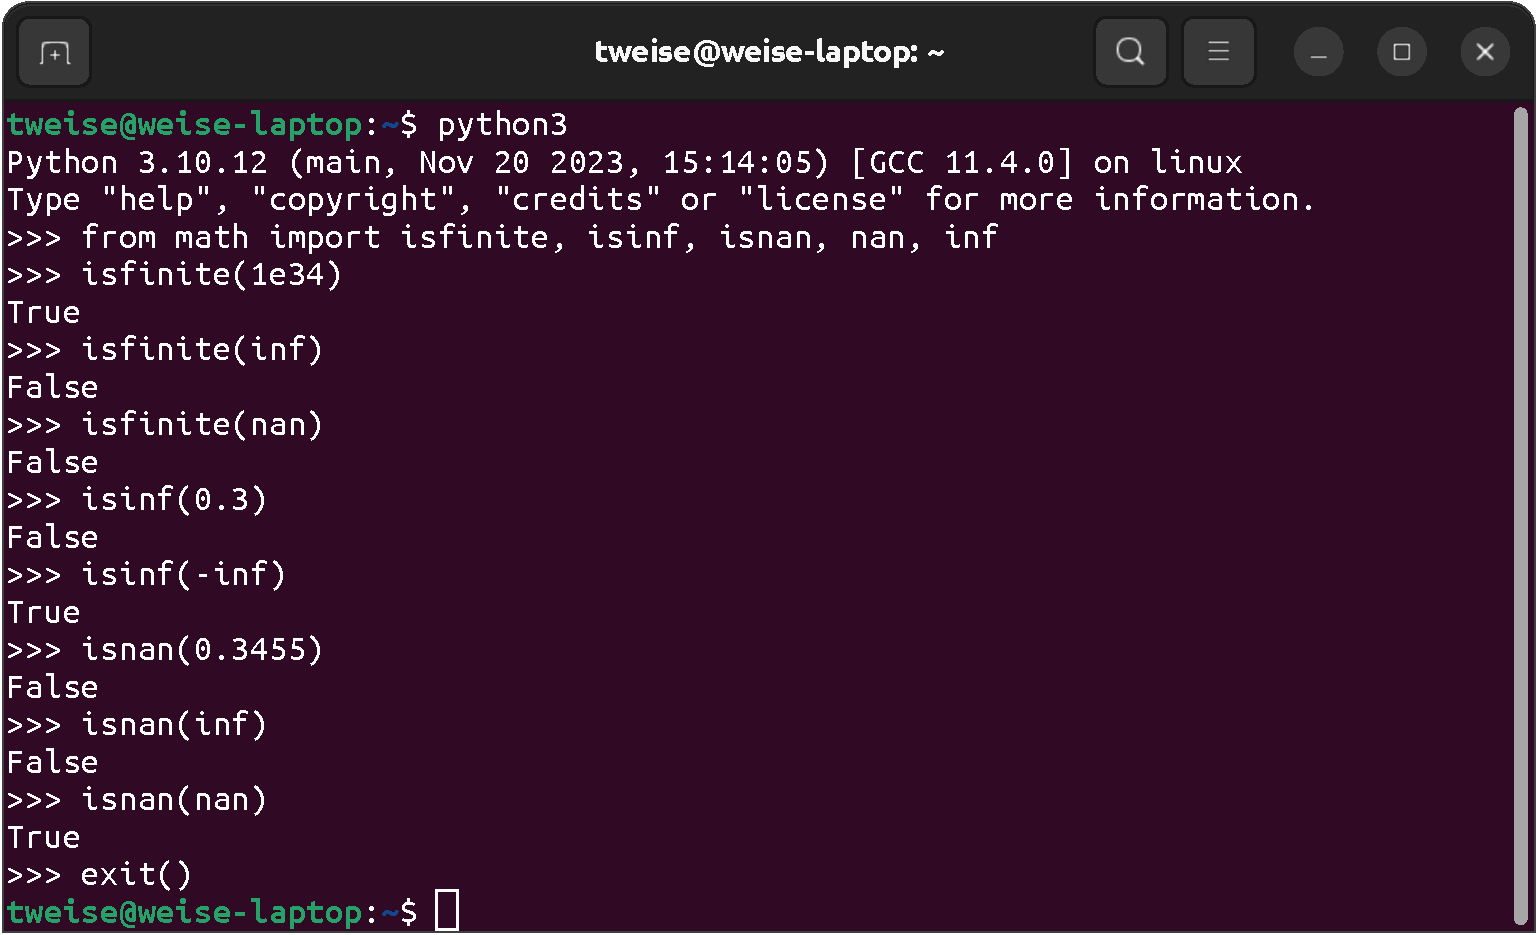
\includegraphics[width=0.8\linewidth]{\currentDir/floatMathInConsoleCheckFinite}%
\caption{Checking for \pythonilIdx{nan} and \pythonilIdx{inf} via \pythonilIdx{isfinite}, \pythonilIdx{isinf}, and \pythonilIdx{isnan}.}%
\label{fig:floatMathInConsoleCheckFinite}%
\end{figure}%

Either way, the possible occurrence \pythonilIdx{inf} and \pythonilIdx{nan} in floating point computations is a cumbersome issue.
If we want to further process results of a computation, we often want to make sure that it is neither \pythonilIdx{inf} nor \pythonilIdx{-inf} nor \pythonilIdx{nan}.
This can be done via the function \pythonilIdx{isfinite}, which we can import from the \pythonilIdx{math} module\pythonIdx{import}\pythonIdx{from}, as you can see in \cref{fig:floatMathInConsoleCheckFinite}.
\pythonil{1e34} is a large number, but \pythonil{isfinite(1e34)} is certainly \pythonilIdx{True}.
\pythonil{isfinite(inf)} and \pythonil{isfinite(nan)} are both \pythonilIdx{False}.
The function \pythonilIdx{isinf}, again from the \pythonilIdx{math} module, checks if a \pythonilIdx{float} is infinite.
\pythonil{isinf(0.3)} is therefore \pythonilIdx{False} whereas \pythonil{isinf(-inf)} is \pythonilIdx{True}.
Finally, we can check whether a \pythonilIdx{float} is \pythonilIdx{nan} via the \pythonilIdx{isnan} function from the \pythonilIdx{math} module.
\pythonil{isnan(0.3455)} and \pythonil{isnan(inf)} are both \pythonilIdx{False}, whereas \pythonil{isnan(nan)} is \pythonilIdx{True}.%
%
\endhsection%
%
\hsection{Summary}%
%
In many situations, integer numbers are the way to go, for example when we count things or add discrete quantities.
However, fractional numbers are also very common and we encounter them all the time in our daily life.
Fractional numbers can be represented by the \pythonilIdx{float} datatype in \python.

\python\ offers us the very cool feature that basically arbitrary integer numbers can be represented by the \pythonilIdx{int} datatype.
We can store very large numbers and are only limited by the memory available on our computer.
Very large integer numbers are, however, something of a corner case {\dots} they do not happen often.

Real numbers in~\realNumbers\ are a whole different beast.
They include irrational numbers like~$\sqrt{2}$ and transcendental numbers like~$\pi$.
These numbers are needed \emph{often} and they have infinitely many fractional digits.
Thus, there is no way to exactly represent them in computer memory exactly.
Another problem is that we may need both very large numbers like~$10^{300}$ and very small numbery like~$10^{-300}$.

Floating point numbers~\cite{G2023CAIP}, provided as the \python\ datatype \pythonilIdx{float}, solve all of these problems (to some degree).
They offer a precision of about 15~digits for a wide range of large and small numbers.
15~digits are more than enough for most applications.
Many functions for floating point numbers, like logarithms and trigonometric functions, are offered by the \pythonilIdx{math} module.

Floating point numbers can be converted back to integers via rounding or truncating.
Since writing out numbers such as $5.235^{212}$ in their full length would waste a lot of space and also make no sense, since only the highest 15~digits are actually stored and the rest would be random nonsense, the scientific notation was developed.
It would represent this number as \pythonil{5.235e+212}, which is quite readable if you know that the~\pythonil{e} in \pythonil{eXXX} here just means~$10^{\mathtt{XXX}}$.

However, when one deals with floating point numbers, a set of nasty problems can occur.
For example, it could happen that we want to represent a number which is just \emph{too big} of the available range.
This number would be rendered as \pythonilIdx{inf}, which stands for both mathematical infinity~$\infty$ and, well, \inQuotes{too big to be represented}.
In some cases, computations that would exceed the available range may also raise an \pythonilIdx{OverflowError}, which simply terminates them (we learn about this later).
Numbers which are too tiny, on the other hand, simply become~\pythonilIdx{0}.
Finally, there are also situations where the result of a computation is neither too big nor too small and, yet, not an actual number.
For example, a way to make mathematicians cry would be to try to compute \pythonil{inf - inf} or \pythonil{inf / inf}.
The result is then \pythonilIdx{nan}, i.e., \inQuotes{Not a Number}\pythonIdx{Not a Number}.
The value \pythonilIdx{nan} has the interesting property that it is (to my knowledge) the only native \python\ value which is \emph{different from itself}, i.e., \pythonil{nan != nan}.
The \pythonilIdx{math} module offers a set of functions to check whether a value is finite~(\pythonilIdx{isfinite}), infinite~(\pythonilIdx{isinf}), or \pythonil{nan}~(\pythonilIdx{isnan}).

When doing floating point computations, these are the issues that you should aware about.
The precision and range is limited and strange things happen at these limits.%
%
\endhsection%
%
\endhsection%
%
